% -*- TeX-master: "Qualificacao.tex" -*-
%!TEX root = Qualificacao.tex

\chapter{Controller Structure Selection}\label{cap:CCS}
\vspace{-1cm}

% Frase citação inicial {{{1
% \begin{flushright}
% \begin{minipage}{0.7\linewidth}
%     \emph{``\dots''}
% \end{minipage}
% \end{flushright}
%
% \begin{flushright}
% Cicrano
% \end{flushright}
%
%\vspace{1cm}

% Intro CAP {{{2

Neste capítulo, são apresentadas propostas para projeto de controladores DDC no que diz respeito à escolha de estrutura do controlador. A metodologia utilizada, assim como os resultados Preliminares obtidos em uma primeira etapa de testes são apresentados.

Nesta pesquisa, o foco tem sido dado ao estudo e desenvolvimento de técnicas de seleção de estruturas para o modelo de controladores realimentados em procedimento de projeto DDC\@.
A intenção é, no âmbito de controle de sistemas não lineares, adaptar técnicas de seleção de estruturas conhecidas na área de identificação de sistemas para lidar com o caso de controle, onde neste caso, o sistema a ser identificado, passa a ser o controlador. Para atingir estes objetivos optou-se pelo uso de modelos polinomiais para representação dos controladores, inicialmente com estruturas NARX\@. Esta escolha é conveniente devido à característica de flexibilidade estrutural e a capacidade desses modelos em descrever sistemas não lineares~\citep{pearson1999,martins2013}.
% \begin{figure}[htpb]
    % \centering
    % \missingfigure{Pretendo colocar por aqui um diagramas (deve ser blocos) para ajudar.}
    % % \includegraphics[width=0.8\textwidth]{}
    % \caption{}
    % \label{fig:Diagrama representativo}
% \end{figure}
%

Como mencionado no Capítulo~\ref{cap:cap2}, uma das principais etapas no procedimento de identificação de sistemas a partir de dados é a etapa de escolha do modelo. Trabalhos que visam dar uma luz a esta tarefa têm sido propostos, como o caso dos trabalhos desenvolvidos por~\cite{falsone2014,falsone2015} em que uma abordagem aleatória é utilizada a fim de selecionar os melhores candidatos entre os possíveis regressores na formação do modelo a ser identificado.

% As mentioned in Chapter~\ref{cap:cap2}, one of the main steps in the procedure of model system identification from data is the model selection step.  Studies that aim to deal with this task have been proposed, as is the case of studies developed by~\cite{falsone2014, falsone2015} in which a random approach, named RaMSS, is used in order to select the best candidates to compose a final model structure, among a class of possible regressors.

% \todo{Confirmar se o RaMSS original só é aplicável a NARX mesmo na sua forma original. Se for, falar aqui.}
Mais recentemente,~\cite{retesNARMAXModelIdentification2019} estenderam a estratégia RaMSS para escolha de estruturas de modelos NARMAX, que levam em conta o efeito de ruídos nos sinais no intuito de reduzir a polarização nas estimativas paramétricas. 
\todo{Colocar aqui mais referências neste sentido. Seleção de estruturas.} 

No âmbito de projeto de controladores baseado em dados, mais especificamente pelo método VRFT, em que o os parâmetros do controlador são ajustados por técnicas de identificação convencionais como OLS, ILS, IV, dentre outras, o mesmo problema de escolha de estrutura do modelo ocorre, com a diferença que agora o modelo representa o controlador, e não mais o processo. Portanto, analogias devem poder serem feitas em relação ao uso do método RaMSS no intuito de estendê-lo para fins de identificação da estrutura mais adequada para o controlador.

Neste sentido, o presente trabalho tem se voltado ao estudo das possibilidades e consequências do uso dessas tecnologias para escolha da estrutura do controlador que se mostre mais adequada para fins de controle. Como metodologia para atingir este objetivo, listam-se as etapas a seguir, que por sua vez são detalhadas nas seções subsequentes:
\begin{itemize}
    \item O método RaMSS, como concebido originalmente, é implementado em ambiente computacional e a partir de simulações de processos deseja-se certificar de que a metodologia apresenta bons resultados para identificação de processos, além de garantir que algoritmo esteja funcionando de acordo com o esperado. Alguns resultados são brevemente analisados.
    \item O algoritmo utilizado na etapa anterior é usado, na sequência, para primeiros testes de projeto de controladores a partir da estratégia VRFT sem modificações significativas em seu mecanismo. Neste cenário se espera alguns primeiros resultados, mas sem maiores compromissos com resultados satisfatórios, mas de grande valia para análise e comparação das modificações propostas. Respostas para sistemas previamente definidos são analisados.
    \item Como passo seguinte, modifica-se o cálculo do índice de custo responsável pelo cálculo dos RIP do algoritmo RaMMS, visando adaptar estes índices para fins de controle.
    \item Na sequência apresenta-se um estudo a respeito do uso de informações auxiliares durante o projeto do controlador, como introdução de restrições durante a etapa de identificação que garantam características desejáveis e previamente definidas na malha fechada.
\end{itemize}

Por fim, discussões a respeito de estabilidade, convergência, polarização e robustez são apresentadas, ainda não em um contexto de garantias, mas como conjecturas de passos que pretende-se aprofundar na sequência da presente pesquisa.

\section{Methodology}\label{sec:CSS_metod}


\section{Preliminary Results}\label{sec:prel_results}


% \begin{exmp}[Motor de corrente contínua] Considere um motor de corrente contínua, com modelo simplificado dado pela equação diferencial
% \begin{equation}
% \label{eq:motorccss}
    %
% \end{equation}
% \end{exmp}
\begin{exmp}[Sistema linear de 2a ordem]\label{ex:sis2aord}
    Considere o seguinte sistema linear de segunda ordem no tempo discreto:
    \begin{equation}
    \label{eq:sis2aord}
        y_k = a_1y_{k-1} + a_2y_{k-2} + b_1u_{k-1} + b_2u_{k-2},
    \end{equation}
    onde, para $i = 1,\ 2$, os termos $a_i$, $b_i$ $\in \R$, representam parâmetros constantes; $u_{k-i}$ e $y_{k-i}$ $\in \R$, os sinais de entrada e saída, respectivamente; e $k$ o índice temporal.
    De acordo com a estratégia VRFT (Capítulo~\ref{cap:VRFT}), deve-se primeiramente definir uma classe de controladores admissíveis $\mathscr{C}$, contendo a estrutura do controlador desejado, e definir um modelo de referência que expresse o comportamento do sistema em malha fechada desejado.

    A fim de se examinar o comportamento do Algoritmo RaMSS em achar o melhor conjunto de parâmetros, procede-se da seguinte maneira:

    Define-se um modelo de referência 
    \todo{não estou certo se posso usar esta palavra ``factível''.}
    factível, ou seja com grau relativo igual ou superior ao do processo. Por simplicidade, escolhe-se um modelo de 1a ordem com mesmo grau relativo, dado pela função de transferência
 \begin{equation}
    T_d(z) = \frac{1-A}{z-A},
    \label{eq:mr_sis2aord}
 \end{equation}
    sendo $A$ um parâmetro de projeto relacionado a constante de tempo do sistema por  $A = \frac{T_s}{\tau_d}$, sendo $T_s$ o período de amostragem e $tau_d$ a constante de tempo desejada.

    Como nesse exemplo teórico o modelo do processo é completamente conhecido, o controlador compatível (ideal), pode ser calculado facilmente por~\ref{eq:control_ideal}, o que resulta, no domínio do tempo, na seguinte equação de diferenças
    \begin{equation}
    \label{eq:contIdeal_sis2aord}
        m_k = \theta_0e_{k} + \theta_1e_{k-1} + \theta_2e_{k-2} + \theta_3m_{k-1} + \theta_4m_{k-2},
        % # umf[k] <- 10.38*emf[k] - 16.66*emf[k-1] + 6.957*emf[k-2] - ( - 0.125*umf[k-1] - 0.875*umf[k-2] )
    \end{equation}
    em que $m_k \in \mathbb{R}$ e $e_k \in \mathbb{R}$ representam respectivamente os sinais de controle e erro de rastreamento no instante $k$, e $\theta_i$, com $i=1,2,3,4$, os parâmetros do controlador.
    Adotando, $ a_1 = a_2 = b_1 = b_2 = A = \tau_d = T_s = 1$,
    \todo{Corrigir aqui estes parâmetros, não é isso no discreto (acho que os índices adotados foram no contínuo.). Na verade melhorar toda a frase.} como parâmetros para os modelos de processo e de referência, e através de~\eqref{eq:control_ideal} e~\eqref{eq:contIdeal_sis2aord} chega-se ao vetor de parâmetros $\vtheta$ para o controlador ideal, definido como
 \begin{equation}
     \vtheta^T = \begin{bmatrix} \theta_0 & \theta_1 & \theta_2 & \theta_3 & \theta_4 \end{bmatrix}^T =  \begin{bmatrix} 
      10.38 & -16.66 & 6.957 & 0.125 & 0.875 \end{bmatrix}^T
    \label{eq:}
    \end{equation}
    Utilizando o algoritmo RAmSS, como abordado na seção~\ref{sec:ramss}.
    O procedimento é executado para 2 casos:
    \begin{description}
        \item[caso 1] o conjunto universo $\mathscr{M}$ é tomado como todos os possíveis modelos lineares formados pelos regressores com até 4 e 6 atrasos temporais para o sinal de entrada (erro virtual, $\overline{e}_k$) e saída (sinal de excitação do processo, $u_k$), respectivamente. Os parâmetros de simulação apresentados na tabela~\ref{tab:sis2aord}. 
        \item[caso 2] o conjunto universo $\mathscr{M}$ é tomado como todos os possíveis modelos \textit{não lineares} formados pelos mesmos regressores do caso anterior. 
        % \item[caso 2] o conjunto universo $\mathscr{M}$ é tomado como todos os possíveis modelos \textit{não lineares} formados pelos regressores com até 4 e 6 atrasos temporais para o sinal de entrada (erro virtual, $\overline{e}_k$) e saída (sinal de excitação do processo, $u_k$), respectivamente.
    \end{description}
    Os parâmetros de simulação para os 2 casos são apresentados na tabela~\ref{tab:sis2aord}. 

\begin{table}[htpb]
    \centering
    \caption{Parâmetros para simulação do algoritmo RaMSS do exemplo~\ref{ex:sis2aord} }\label{tab:sis2aord}
    \begin{tabular}{c|c|c|c|c|c|c|c}
        Caso & $o$ & $n_e$ & $n_m$ & $N_p$ & $N_i$ & $K_J$ & $\gamma$ \\
        \hline
        1 & $ 1 $ & $7$ & $4$ & $100$ & $100$ & $1$ & $0.1$ \\
        2 & $ 2 $ & $7$ & $4$ & $100$ & $100$ & $1$ & $0.1$
    \end{tabular}
\end{table}
\todo{Estou pensando em colocar a tabela em apêndice, com significado dos símbolos apresentados por lá.}

Os seguintes  controladores são encontrados para o casos 1 e 2,
% \begin{align}
    % \overline{\vtheta}_1^T  &= \begin{bmatrix}  &  &  &  &  \end{bmatrix}^T  \\
    % \overline{\vtheta}_2^T &= \begin{bmatrix}  &  &  &  &  \end{bmatrix}^T
    % \label{eq:parEst_sis2aord}
% \end{align}

\begin{align*}
   \label{eq:contEst_sis2aord}
   m_1(k) &= 10.0707145 e_1(k) - 16.2413162 e_1(k-1) + 6.8274122 e_1(k-3) \\ &\quad + 0.1941415 m_1(k-1) +  0.8059737 m_1(k-2), \\
   m_2(k) &= 3.4128550 e_2(k) - 3.2267597e_2(k-1) + 0.5117530 m_2(k-1) +  0.4807692m_2(k-2),
\end{align*}
onde o índice subscrito nas variáveis representam os respectivos casos.

% A figura~\ref{fig:fig:sis2aord_RIPs} mostra a evolução dos RIPs para os 2 casos.
% \begin{figure}[htpb]
    % \centering
    % \includegraphics[width=1\textwidth]{sis2aord2_RIP.png}
    % \caption{Evolução dos índices de Probabilidades de inclusão dos regressores para o caso 2 }
    % \label{fig:sis2aord_RIPs}
% \end{figure}

\begin{figure}[H]
    \centering
    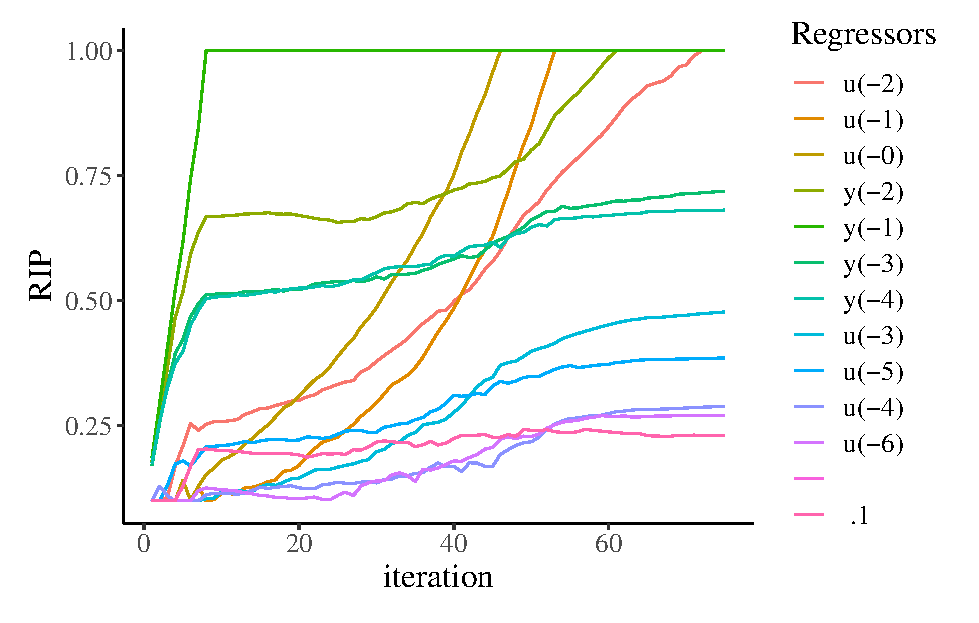
\includegraphics{Figs/sis2aord_l_ramss_RIPs.eps}
    \caption{Evolução dos RIPs para escolha dos regressores para o caso 1.}
    \label{fig:sis2aord_RIPs_caso1}
\end{figure}
\begin{figure}[H]
    \centering
    \includegraphics{Figs/sis2aord_nl_ramss_RIPs.eps}
    \caption{Evolução dos RIPs para escolha dos regressores para o caso 2.}
    \label{fig:sis2aord_RIPs_caso2}
\end{figure}
% \begin{figure}[H]
    % \centering
    % % \subfloat[\centering]{{\includegraphics[width=8cm]{Figs/sis2aord_RIPs_l.png} }}%
    % % \subfloat[\centering]{{\includegraphics[width=8cm]{Figs/sis2aord_RIPs_nl.png} }}%
    % \subfloat[\centering]{{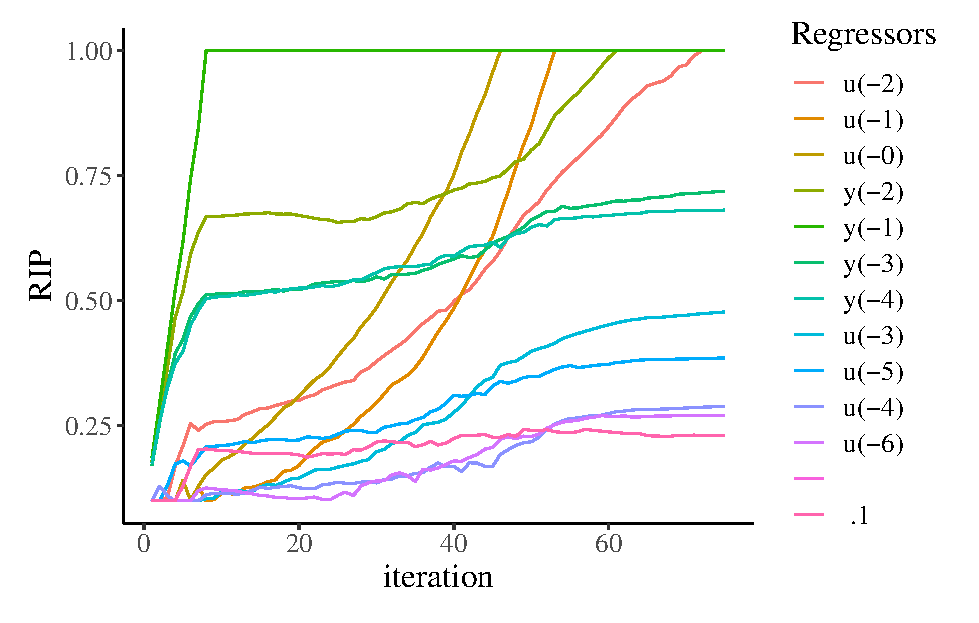
\includegraphics[width=8cm]{Figs/sis2aord_l_ramss_RIPs.eps} }}%
    % \subfloat[\centering]{{\includegraphics[width=8cm]{Figs/sis2aord_nl_ramss_RIPs.eps} }}%
    % \caption{Evolução dos RIPs para escolha dos regressores para os casos (a) 1 e (b) 2.}
    % \label{fig:sis2aord_RIPs}
% \end{figure}



A figura~\ref{fig:Figs-RespostaSist2aordNARX-png} mostra a resposta temporal para os 2 casos.
\begin{figure}[H]
    \centering
    \includegraphics[width=1\textwidth]{Figs/sis2aord2-cropped.pdf}
    \caption{Resposta temporal a um sinal de referência a um sinal de referência (preto tracejado) na forma de degraus para o modelo de referência em~\eqref{eq:mr_sis2aord} (preto contínuo) e para um possível modelo escolhido pelo algoritmo RaMSS (azul contínuo).}
    \label{fig:Figs-RespostaSist2aordNARX-png}
\end{figure}

\todo[inline,color=cyan]{\textbf{To LAA: } Aguirre, peço desculpas pelas figuras ainda com legendas e com qualidades não vetoriais. Ainda não pesquisei um método efetivo para produzir figuras melhores. Uma alternativa fácil para mim é plotar pelo Matlab. Mas creio que pelo R será tranquilo também. Mas só devo ajustar as figuras lá para o final de semana.} 
 
Nota-se que, ao se considerar somente termos lineares como candidatos, o algoritmo converge para o conjunto de regressores do caso ideal, porém o mesmo não ocorre quando se considera o caso com termos não-lineares. Mesmo ao repetir o procedimento de forma aleatória e exaustiva, o resultado permanece parecido, convergência para a estrutura ideal para o caso 1 e praticamente todos os casos e convergência para diferentes estruturas, que muitas vezes não condiz com o caso ideal.

Este exemplo serve como base para mostrar o comportamento do RaMSS quando utilizado diretamente ao projeto VRFT\@. Porém nenhuma adaptação é feita a fim de lidar com seleção de estruturas de controlador especificamente.

\end{exmp}


\todo[color=cyan]{\textbf{To LAA: } O exemplo anterior está mal terminado. Estava trabalhando nele agora por último. Mas estou cansado e estou vendo que piorando mais do que melhorando. Então estou enviando o arquivo do jeito que está.} 

\todo[inline]{Estou querendo colocar ainda uma análise ``mais estatística'' da seleção dos modelos. Como neste exemplo, nem sempre os regressores escolhidos são os mesmos, principalmente para o ``caso 2''. A ideia é fazer uma espécie de histograma, considerando várias realizações. Chegui a fazer o hitograma, mas depois percebi que não era exatamente um histograma, mas algo parecido que quero.} 
% \todo[color=cyan]{\textbf{To LAA: } Quis fazer um exemplo simples para começar, acabou me tomando mais tempo do que deveria. A ideia seria apresentar alguns exemplos (ao longo de uma metodologia que ainda está faltando), primeiramente este, que mostra a aplicação direta do RaMSS ao problema sem modificações. Queria dar uma motivação para usar mudanças propostas. Quero apresentar na sequência um exemplo usando o erro de rastreamento no calculo do RaMSS. Ainda não estou com o resultado totalmente pronto. Decidi tentar colocar uma restrição para garantir um integrador mas os resultados não foram muito animadores. Mas acho que já percebi por que e creio que usando informação do erro de rastreamento isso pode melhorar.}

\todo{Colocar aqui sobre as modificações introduzidas no RaMSS a fim de lidar com a identificação do controlador. Aprveitar e batizar o método de RaCSS.} 

% \section{RAmSS aplicado a um sistema linear de 2$^a$ ordem}\label{sec:}
% \todo[inline]{Neste exemplo aplico o ``RaCSS''a um sistema de 2a ordem, usando informação do erro de rastreamento no cálculo dos RIPs.}

\begin{exmp}[RaCSS aplicado a um sistema linear de 2$^a$ ordem]

Neste exemplo aplico o ``RaCSS'' ao mesmo sistema de 2a ordem do exemplo anterior, mas agora usando informação do erro de rastreamento no cálculo dos RIPs.

Por enquanto coloquei basicamente os gráficos dos resultados. O texto será colocado na sequência.

\begin{figure}[H]
  \centering
  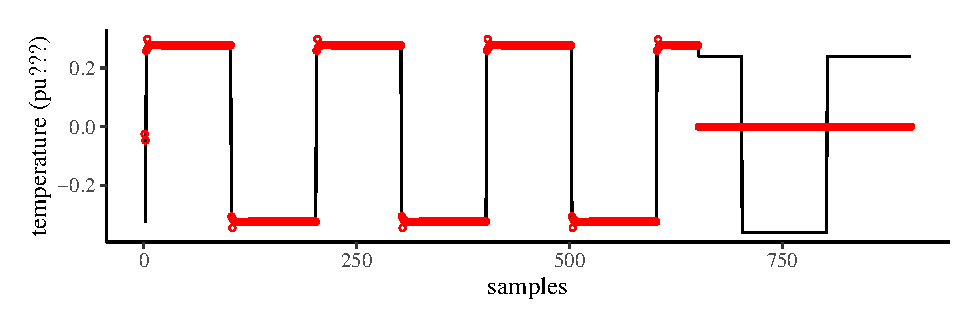
\includegraphics{./Figs/s.motorcc.VRFT.racss_train_val_data.eps}
  \caption{Dados de treinamento (até a amostra 700) e validação (a partir da amostra 700).}\label{fig:RIPs2}
\end{figure}
\todo[inline]{Os dados de validação estão com problemas, mas foi alguma coisa errada na hora de plotar. Obviamente irei consertar isso. Também não estou muito certo se coloco ou não estes dados.} 

\begin{figure}[H]
  \centering
  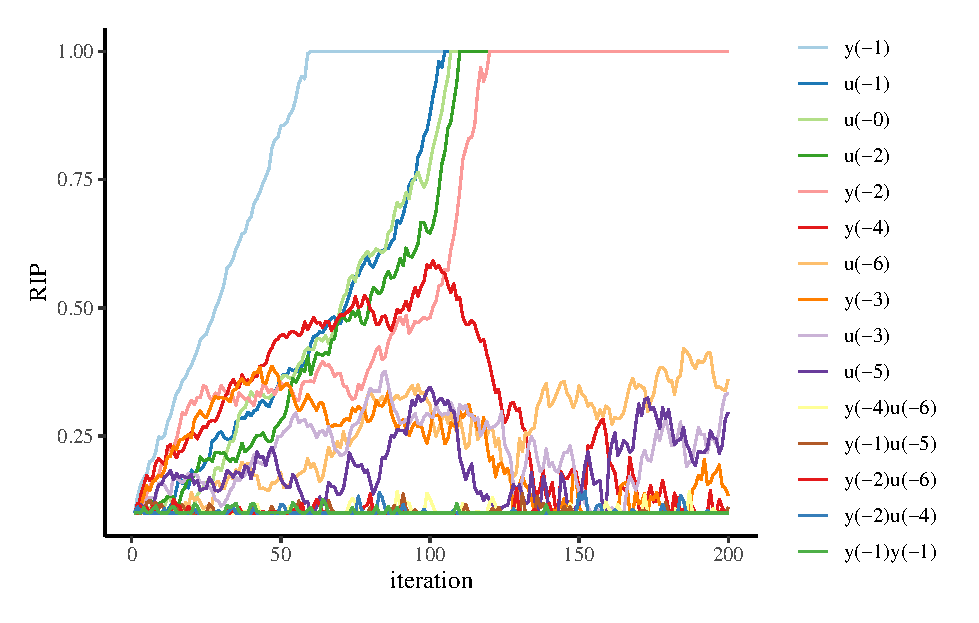
\includegraphics{./Figs/s.motorcc.VRFT.racss_RIPs.eps}
  \caption{Evolução dos RIPs para a estratégia RaCSS aplicada ao modelo linear de 2a ordem.}
  \label{fig:RIPs2}
\end{figure}

\begin{figure}[H]
  \centering
  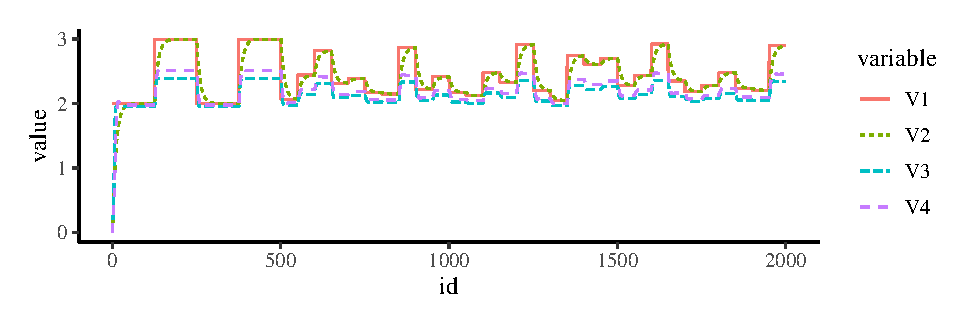
\includegraphics{Figs/s.heater.var.dissip.VRFT_teste.eps}
  \caption{Figura de teste.}
  \label{fig:teste}
\end{figure}

\begin{figure}[H]
  \centering
  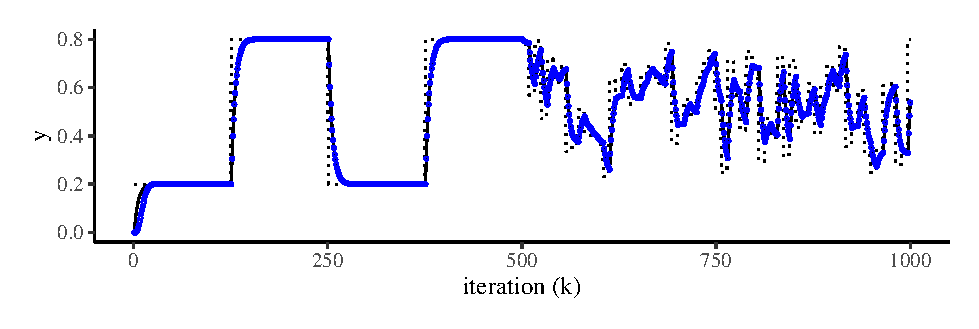
\includegraphics{./Figs/s.motorcc.VRFT.racss_output.mf.eps}
  \caption{Resposta em malha fechada ao sinal de referência (pontilhado preto), para o modelo de referência (preto contínuo) e para o controlador obtido usando a estratégia RaCSS (círculo azul).}
  \label{fig:}
\end{figure}

Interessante notar que agora, mesmo usando regressores não-lineares, o que aumenta a possibilidade de modelos, a estrutura do modelo converge para a estrutura ideal, que é linear neste caso


\end{exmp}


\begin{exmp}[RaCSS aplicado a um sistema não-linear]
   Neste exemplo a ideia é avaliar o comportamento do ``RaCSS'' a um sistema não-linear. Quero tomar o mesmo modelo de um aquecedor com dissipação variável adotado no exemplo~\ref{ex:varHeater} da seção~\ref{sec:ramss}

\todo[inline]{Estava tentando colocar estes resultados aqui agora, mas está dando algum erro no algoritmo. Como está em cima da hora da nossa reunião, vai ficar assim.}
% Por enquanto coloquei basicamente os gráficos dos resultados. O texto será colocado na sequência.
%
% \begin{figure}[H]
  % \centering
  % 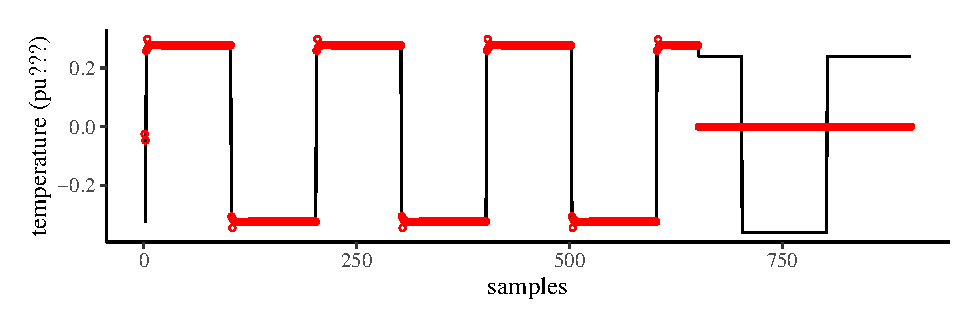
\includegraphics{./Figs/s.motorcc.VRFT.racss_train_val_data.eps}
  % \caption{Dados de treinamento (até a amostra 700) e validação (a partir da amostra 700).}
  % \label{fig:RIPs2}
% \end{figure}
% \todo[inline]{Os dados de validação estão com problemas, mas foi alguma coisa errada na hora de plotar. Obviamente irei consertar isso.}
%
% \begin{figure}[H]
  % \centering
  % 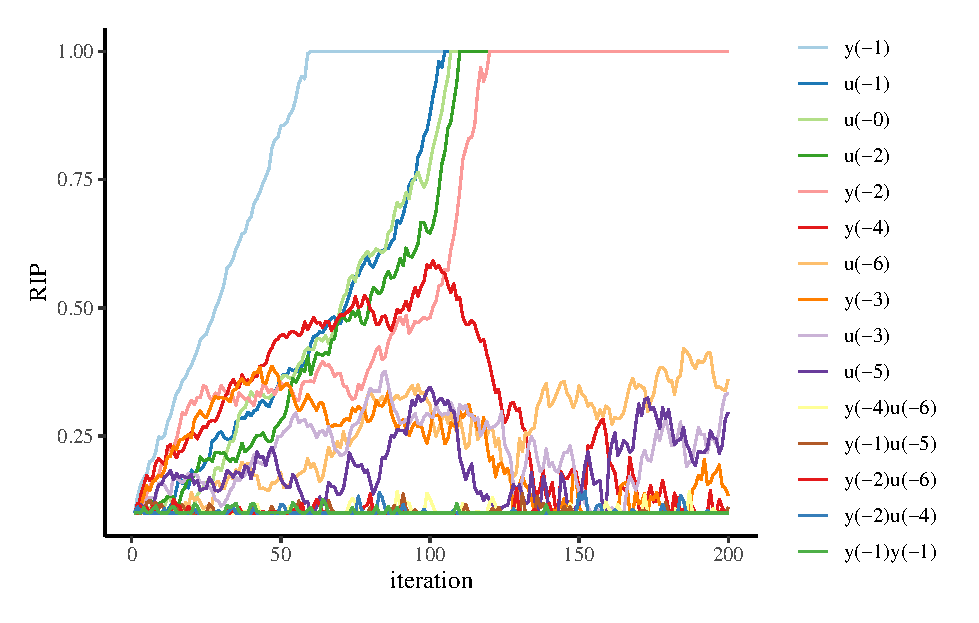
\includegraphics{./Figs/s.motorcc.VRFT.racss_RIPs.eps}
  % \caption{Evolução dos RIPs para a estratégia RaCSS aplicada ao modelo do aquecedor com dissipação variável.}
  % \label{fig:RIPs2}
% \end{figure}
%
% \begin{figure}[H]
  % \centering
  % 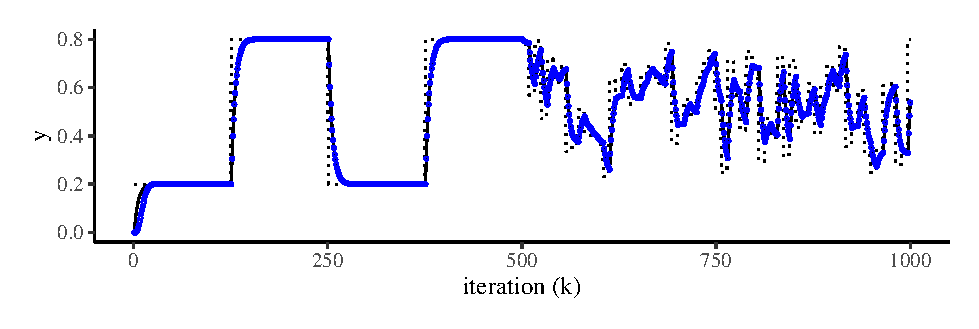
\includegraphics{./Figs/s.motorcc.VRFT.racss_output.mf.eps}
  % \caption{Resposta em malha fechada ao sinal de referência (pontilhado preto), para o modelo de referência (preto contínuo) e para o controlador obtido usando a estratégia RaCSS (círculo azul), considerando o controle de temperatura do aquecedor com dissipação variável.}
  % \label{fig:}
% \end{figure}
%

\end{exmp}
% =================================================================================================================

% \newpage
% \section{Rascunho}\label{sec:Rascunho}
%
%
% Como produto/trabalho em desenvolvimento durante o semestre, cita-se o trabalho que tem sido feito no sentido de desenvolver metodologias para escolha de estruturas para o controlador no âmbito do controle baseado em dados, ou DDC (Data-Driven Control).
% Mais especificamente, tem-se dado ênfase a escolha da estrutura do controlador a partir do uso de métodos VRFT.
% Como deixa claro em seu nome, ao usar o termo “sintonia” (em inglês, “tunning” ), a metodologia VR  FT visa a sintonia de um controlador pertencente a uma classe de controladores pré-estabelecida.
% Como abordado pelos autores do método~\citep{campi2002,campi2006a}, por outros estudiosos do assunto~\citep{bazanella2012} e apresentado neste relatório na seção de revisão bibliográfica, o método visa minimizar o erro de rastreamento de um modelo de referência pré-definido a partir da minimização de uma função de custo.
% Tal função é definida a partir do erro quadrático entre o sinal de excitação utilizado no processo a se controlar e o sinal de controle “virtual”, gerado pelo controlador identificado ao se aplicar  o mesmo sinal de referência capaz de produzir o mesmo sinal de saída  virtual utilizado na identificação.
%~\cite{campi2002} mostram, para o caso linear, e~\cite{campi2006}  e não linear, que ao se minimizar esta nova função de custos, minimiza-se também o erro de rastreamento, desde que se obedeça os seguintes critérios: a classe do controlador considerado tenha uma estrutura que possibilite abrigar o que se nomeia de controlador ideal (vide eq.
% ); que o processo não seja afetado por ruídos; e o controlador seja parametrizado linearmente.
% Caso o controlador ideal não possa ser representado pela classe considerada, o erro mínimo de rastreamento não é mais garantido e a introdução de um filtro ao projeto, visando se aproximar desse mínimo é desejado.
%
%
% No desenvolvimento do trabalho, foco deste relatório, tem-se feito um estudo de como seria possível, e quais as vantagens poderia-se obter se, ao invés de apenas tentar achar a melhor sintonia para um controlador com estrutura pré-estabelecida,  se procurasse também uma melhor estrutura dentro de um um conjunto de classes de controladores, de forma que o erro de rastreamento ótimo ou pelo menos sub-ótimo possa ser encontrado.
%
% Para atingir este propósito, tem-se investigado o uso de técnicas de seleção de estruturas que, com devidas adaptações e reformulações, sejam capazes selecionar modelos que resultem em controladores não lineares (ou mesmo lineares) que possam levar a respostas melhores do que aqueles que fazem uso de estruturas pré definidas.
%
% Dentre as ferramentas que têm-se utilizado, destacam-se o uso da taxa de redução de erro (ERR) e do algoritmo   Randomized Model Structure Selection (RaMSS)~\citep{falsone2014,falsone2015}. Estas estratégias têm sido estendidas e utilizadas em aplicações para determinação de modelos de processos dinâmicos~\citep{retesNARMAXModelIdentification2019} ou até mesmo no projeto de compensadores para aplicações em que o processo exibe determinados efeitos de não linearidade específicas, como no caso de efeitos histeréticos~\citep{abreuIdentificationNonlinearityCompensation2020}.

% Em particular, o método RaMSS, tem se mostrado promissor para a aplicação desejada. Esse método faz apelo às técnicas exploratórias que recorrem a buscas aleatórias ao estilo Monte Carlo, mas com mecanismos de seleção que reduzem drasticamente o custo computacional, evitando uma busca exaustiva, ao mesmo tempo em que tenta garantir uma seleção adequada.
%
% Apoiado nesta técnica, algumas adaptações têm sido estudadas no sentido de lidar agora com a identificação do controlador, e não mais do processo.
%
% Como abordado na revisão bibliográfica deste relatório, o método RaMSS faz uso de um índice de desempenho baseado no cálculo de alguma grandeza que quantifique a qualidade de o modelo em algum sentido. Uma escolha comum é calcular este índice baseado no erro quadrático médio de predição (MSPE).
%
% Um estudo sobre o uso deste índice tem sido feito na pesquisa em questão, conforme resultados apresentados na seção “Análise e Processamento de Dados”. O que se tem observado é que minimizar o MSPE diretamete pela estratégia RaMSS apesar de muitas vezes apresentar bons resultados, não dá garantias que o rastreamento ótimo é alcançado, i.e. aquele em que o erro de rastreamento médio quadrático por exemplo, é mínimo.
%
% Para sanar  esta deficiência, tem-se considerado o uso de algum índice que leve em conta o resultado final ao se aplicar os controladores intermediários identificados e selecionados pelo procedimento. Algo parecido tem sido usado no que diz respeito a identificação de processos  em que o erro quadrático médio de simulação (MSSE) é utilizado em substituição ao MSPE~\citep{aguirre2010}. Neste caso, segundo~\citep{piroddi2003}, o uso de informações da simulação-livre pode melhorar a robustez na seleção de estrutura do processo quando sob condições de identificabilidade parciais.
%
% O MSSE depende da simulação livre, que em suma é a resposta em malha aberta a um sinal de excitação conhecido. Algo parecido poderia ser utilizado ao se avaliar a estrutura no procedimento VRFT, porém, neste caso, seria desejável a resposta do sistema em malha fechada com o controlador obtido a partir da estrutura avaliada. O grande problema neste caso é que esta simulação passa a ser dependente de um modelo, ainda que aproximado do processo. Porém, como estratégias DDC visam exatamente não identificar um modelo para o processo, tal simulação torna-se inviável.
%
% No atual estágio desta pesquisa, tem-se trabalhado com a ideia de um índice que quantifique o erro médio de rastreamento em função do modelo do controlador sintonizado por uma estratégia VRFT, de modo que alguma informação da resposta em malha fechada com o controlador analisado possa ser usada para  o cálculo dos índices de probabilidades de inclusão do regressor, ou RIP (vide seção de Revisão Bibliográfica). Porém, como a simulação da resposta em malha fechada (ou mesmo malha aberta) é inviável devido a uma falta de modelo para o processo, o que se estuda é o uso de técnicas de Aprendizado por Reforço (RL) para que dados colhidos do processo real, enquanto em funcionamento, possam ser usados para o cálculo em tempo real dos RIP e consequentemente para  escolha de melhor estrutura.
%
% Algumas técnicas de RL se mostram promissoras neste caso, uma vez que muitas vezes levam à otimização de índices de desempenho a partir de dados amostrados, sem a necessidade do modelo do processo, ao mesmo tempo em que evitam o alto número de realizações amostrais como em metodologias Monte Carlo. Dentre elas a estratégia TD Learning, tem sido considerada, com uma atenção ao método conhecido como Q-learning, que permite que um controlador possa ser ajustado em uma abordagem conhecida como off-policy. Nesse caso, um controlador ou lei de controle (no caso do presente trabalho, mais precisamente sua estrutura) pode ser determinado enquanto o sistema em malha fechada obedece a uma lei (ou política) de controle diferente. Isto ajuda em eventuais problemas de instabilidade e exploração.
%
% Durante o semestre tem sido desenvolvido um algoritmo no intuito de implementar as ideiais consideradas anteriormente. Parte do algoritmo desenvolvido por Retes (2018), tem sido aproveitada, assim como algoritmos implementados e desenvolvidos pelo grupo do MACSIN1, grupo do qual o autor faz parte desde o início do doutorado. O algoritmo tem sido desenvolvido na linguagem R, portanto traduções de algumas ferramentas já disponíveis no MACSIN em outras linguagens tiveram e estão tendo que ser adaptadas. Os resultados apresentados na seção “Análise e Processamento de Dados” foram obtidos, em sua maioria, a partir deste algoritmo.
